\documentclass{article}
\usepackage{graphicx} % Required for inserting images
\usepackage{amsmath,amssymb,amsthm}
\usepackage{physics}
\usepackage{graphicx,float}
\graphicspath{{images/}}
\usepackage[none]{hyphenat}
\usepackage{blindtext}
\usepackage{parskip}
\usepackage[letterpaper,top=3cm, left= 3cm,bottom=3cm]{geometry}
\usepackage{subcaption}



\title{Fundamental Theorem of Calculus}
\author{Polaris}
\date{2025/04/13}

\begin{document}

\maketitle

\section{Fundamental Theorem of Calculus}
If $f(x)$ is continous on the interval of $[a,b]$, then
\[
\int_{a}^{b} f(x) = F(b) - F(a)
\]
Where $\displaystyle \dfrac{d}{dx}F(x) = f(x)$. This is very powerful, as it links differentiation and integration,
the two fundamental operation in calculus.

Let's take a look at an example question:
\[
\int_{0}^{\frac{\pi}{2}} \cos x \mathrm{d}x
\]
To evaluate this definite integral, we first need to find a function that has a derivative of $\cos x$,
and the function is $\sin x$ (consult back to differentiation), thus by the Fundamental Theorem of Calculus:
\[
    \int_{0}^{\frac{\pi}{2}} \cos x \mathrm{d}x = \sin (\frac{\pi}{2}) - \sin (0) = 1
\]
Where $\displaystyle \sin(\frac{\pi}{2}) = 1$.

\section{Application of FTC}
Let's start with a question, evaluate
\[
\int_{2}^{x}(3t^2-2)\mathrm{d}t
\]
At first glance it seems weird that the variable $x$ is on the upper bound, but let's pretend that $x$ is a number
and do the integral (which is literally algerbra)
\[
\int_{2}^{x} (3t^2-2)\mathrm{d}t = t^3 - 2t \Big|_2^x = x^3 - 2x - 8 +4 = x^3 - 2x -4
\]
This question inspires us to recognize that when a variable is on the integration bound, 
it means the integral will be a function of the variable, or:
\[
\int_{a}^{x} F(t)\mathrm{d}t = f(x) - f(a)
\]
Where again $\displaystyle \dfrac{d}{dx}F(x) = f(x)$ and $f(a)$ is a number.

\newpage
Another way to apply FTC is finding a value of a function at one point with an integral,
let's look at a question:

$F(x)$ is an antiderivative of $f(x)$, if $F(5) = 10$, find an expression that equals to $F(11)$

In order to solve this problem, let's first use FTC:
\[
\int_{5}^{11}f(x)\mathrm{d}x = F(11)-F(5)
\]
Notice here $F(11)$ appears, so we can easily find an expression for $F(11)$:
\[
F(11) = F(5) + \int_{5}^{11}f(x)\mathrm{d}x = 10 + \int_{5}^{11}f(x)\mathrm{d}x
\]

Another way you will see it is in a table:

Consider a function $f(x)$ and its derivative $f'(x)$:
\begin{center}
    \begin{tabular}{||c c c c c||} 
     \hline
     $x$ & $0$ & $2$ & $3$ & $5$\\ [0.5ex] 
     \hline\hline
     $f(x)$ & $-15$ & $-8$ & $4$ & $7$\\ 
     \hline
     $f'(x)$ & 12 & 8 & 3 & -2\\
     \hline
    \end{tabular}
    \end{center}
Find the value of $\displaystyle \int_{0}^{5} f'(x)\mathrm{d}x$

We know that by FTC:
\[
    \int_{0}^{5} f'(x)\mathrm{d}x = f(5) - f(0)
\]
While $f(5) = 7$ and $f(0) = -15$, thus
\[
    \int_{0}^{5} f'(x)\mathrm{d}x = f(5) - f(0) = 7+15 = 22
\]

\newpage
Another way to test about FTC is through graphs:
\begin{figure}[H]
    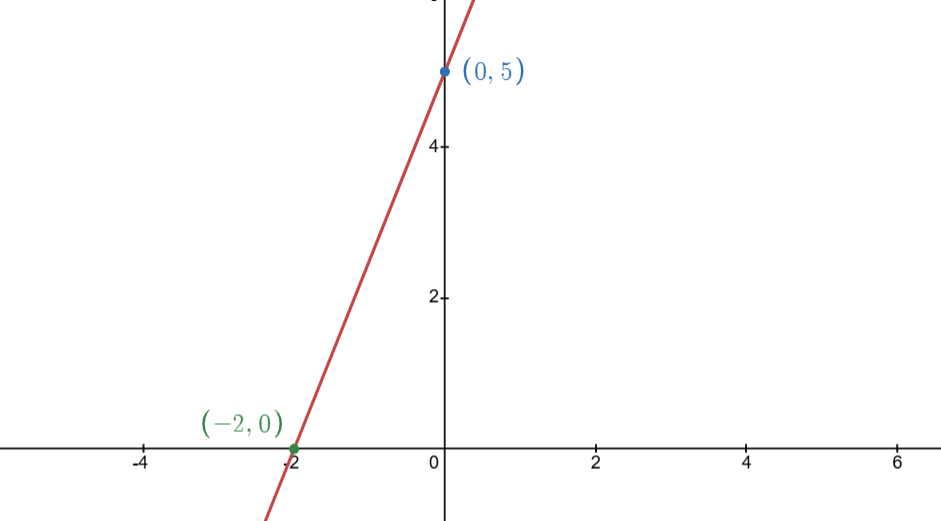
\includegraphics[width = 10cm]{img.png}
    \centering
    \caption{Graph of $f'(x)$}
\end{figure}
Consider a function $f(x)$ with a derivative of $f'(x)$. If this is the graph of $f'(x)$ and $f(-2) = 3$, find $f(0)$.

First, by FTC we have
\[
\int_{-2}^{0}f'(x)\mathrm{d}x = f(0) - f(-2)
\]
Thus
\[
f(0) = f(-2) + \int_{-2}^{0} f'(x)\mathrm{d}x
\]
By the geometric meaning of integrals, $\displaystyle \int_{-2}^{0} f'(x)\mathrm{d}x$ is the area under the curve of $f'(x)$, 
which is the triangle formed by the graph of $f'(x)$ and the coordinate axis.

This offers a way to calculate the integral, the area of the triangle is simply $\displaystyle S = \frac{1}{2}\cdot 2 \cdot 5 = 5$,
thus the integral also equals to $5$, meaning
\[
    f(0) = f(-2) + \int_{-2}^{0} f'(x)\mathrm{d}x = 3 + 5 = 8
\]
The answer is $f(0) = 8$
\end{document}